\chapter{Конструкторский раздел}

\section{IDEF0}

На рисунке~\ref{fig:idef0} приведена диаграмма состояний IDEF0 нулевого уровня, а на рисунке~\ref{fig:idef01} --- диаграмма состояний IDEF0 первого уровня.

\begin{figure}[H]
	\centering
	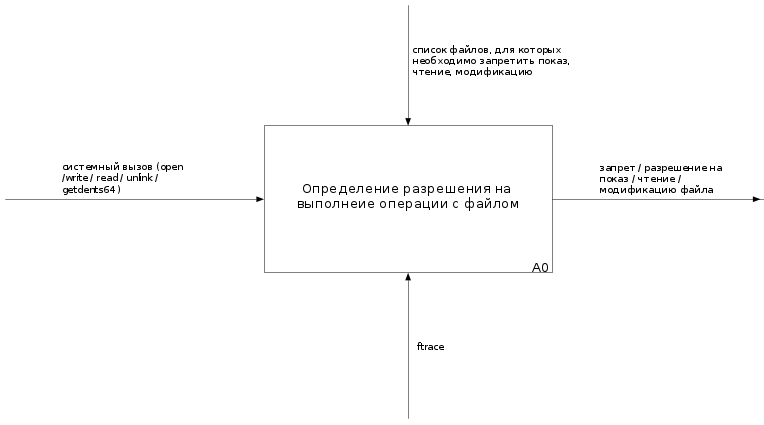
\includegraphics[scale=0.5]{img/01_A0.png}
	\caption{Диаграмма состояний IDEF0 нулевого уровня}
	\label{fig:idef0}
\end{figure}

\begin{figure}[H]
	\centering
	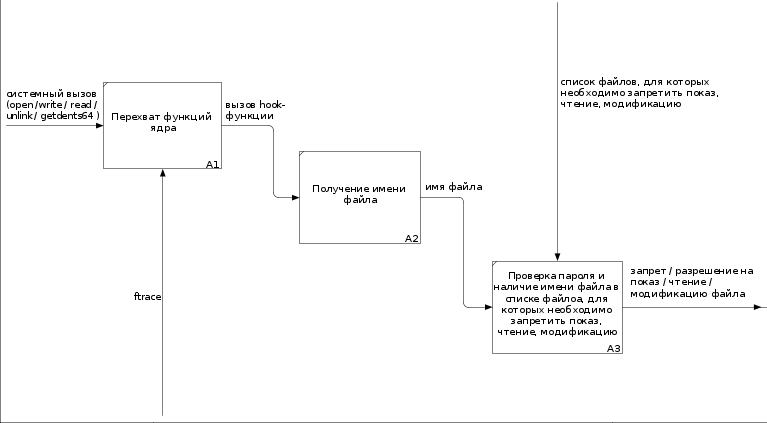
\includegraphics[scale=0.5]{img/02_A0.png}
	\caption{Диаграмма состояний IDEF0 первого уровня}
	\label{fig:idef01}
\end{figure}

\section{Алгоритм проверки необходимости сокрытия файла}

На рисунке~\ref{fig:1} приведена схема алгоритма проверки необходимости сокрытия файла.

\begin{figure}[H]
	\centering
	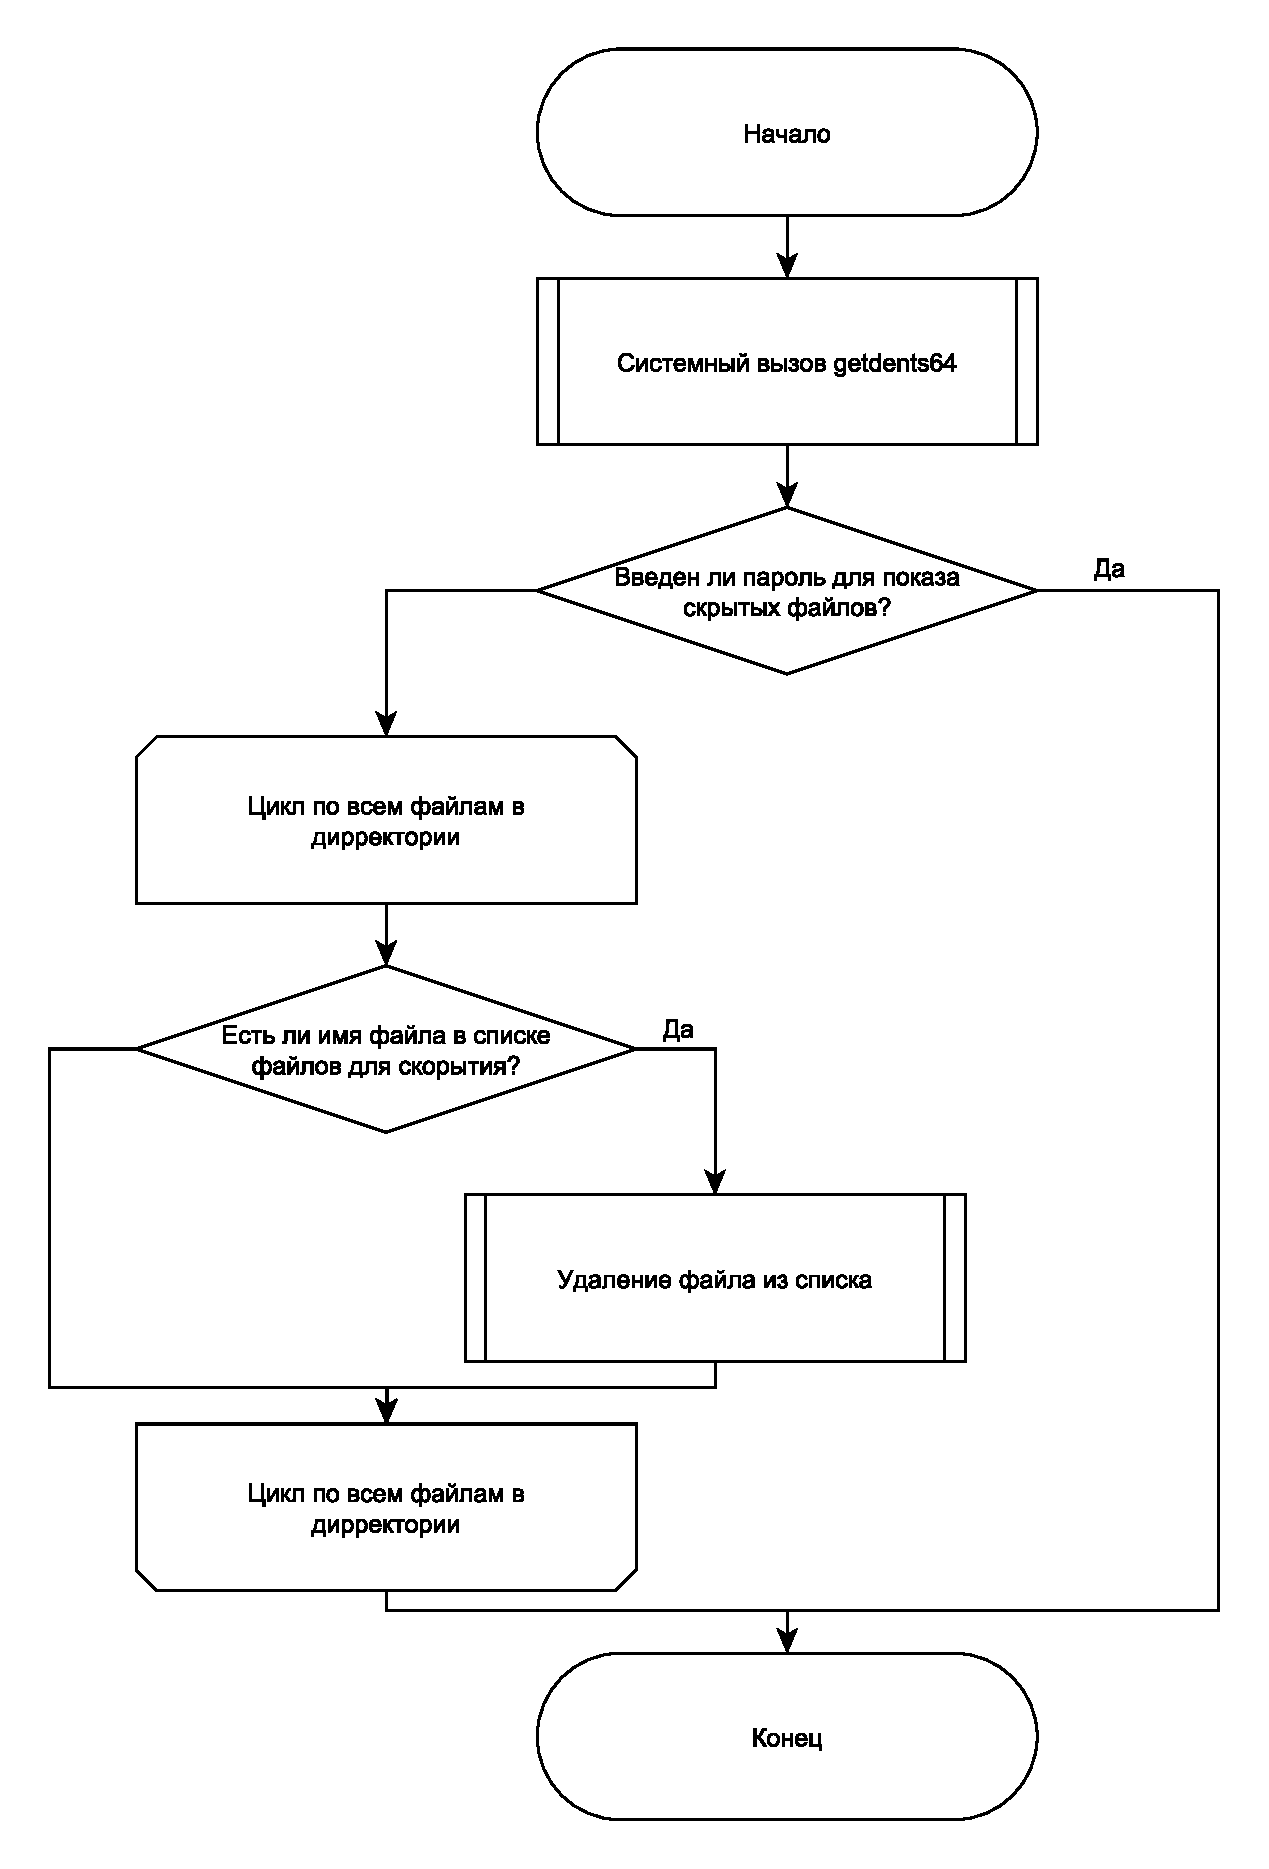
\includegraphics[scale=0.5]{img/first.eps}
	\caption{Алгоритм проверки необходимости сокрытия файла}
	\label{fig:1}
\end{figure}

\section{Алгоритм проверки разрешения на удаление файла}

На рисунке~\ref{fig:2} приведена схема алгоритма проверки разрешения на удаление файла.

\begin{figure}[H]
	\centering
	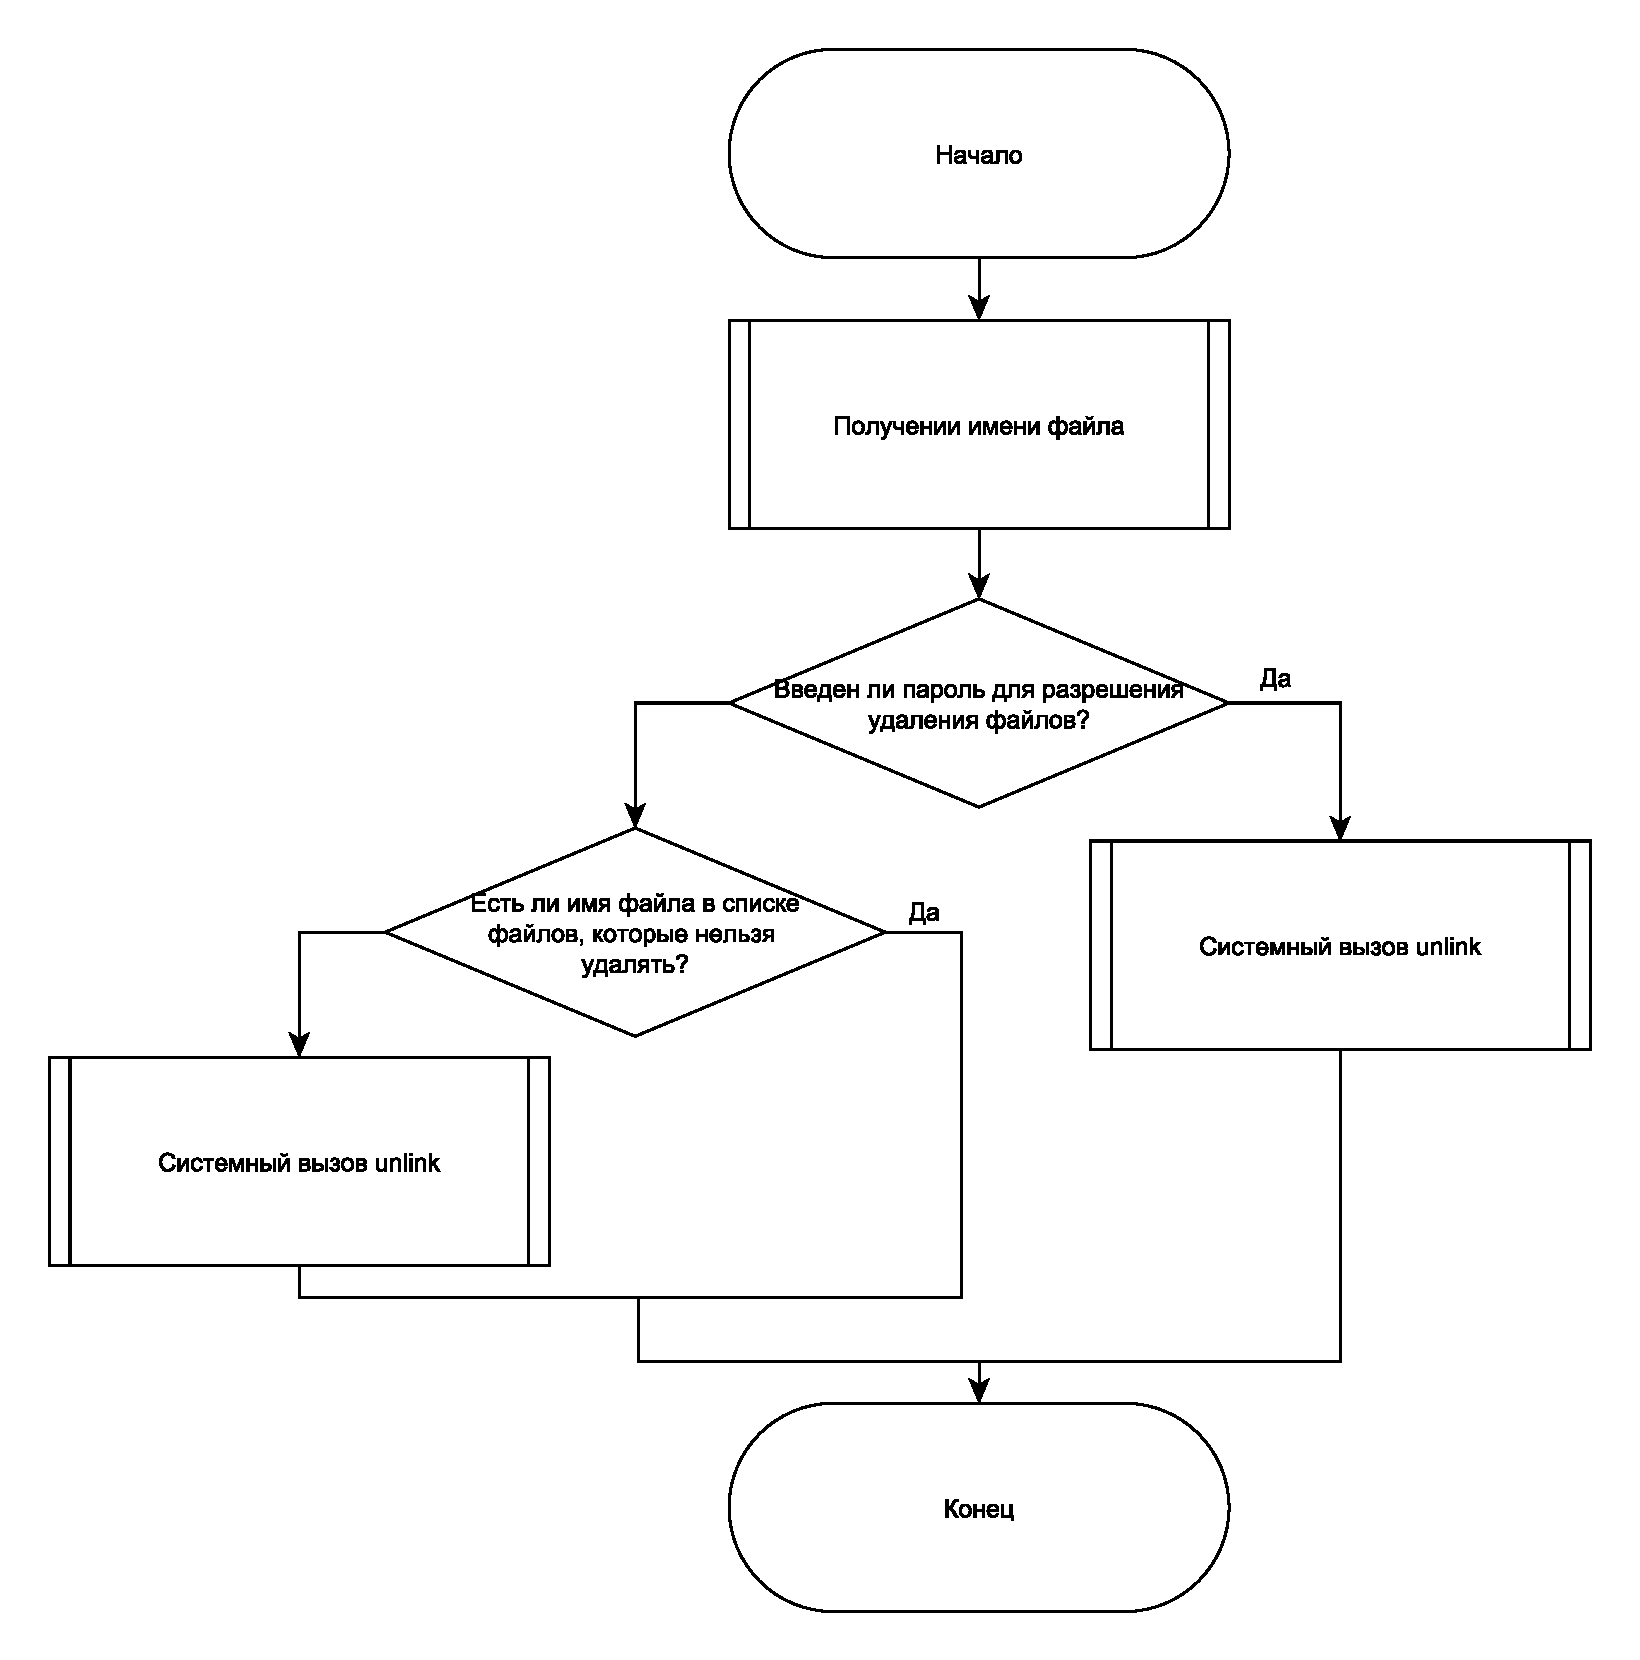
\includegraphics[scale=0.5]{img/second.eps}
	\caption{Алгоритм проверки разрешения на удаление файла}
	\label{fig:2}
\end{figure}

\section{Алгоритм проверки разрешения на запись в файл}

На рисунке~\ref{fig:3} приведена схема алгоритма проверки разрешения на запись в файл.

\begin{figure}[H]
	\centering
	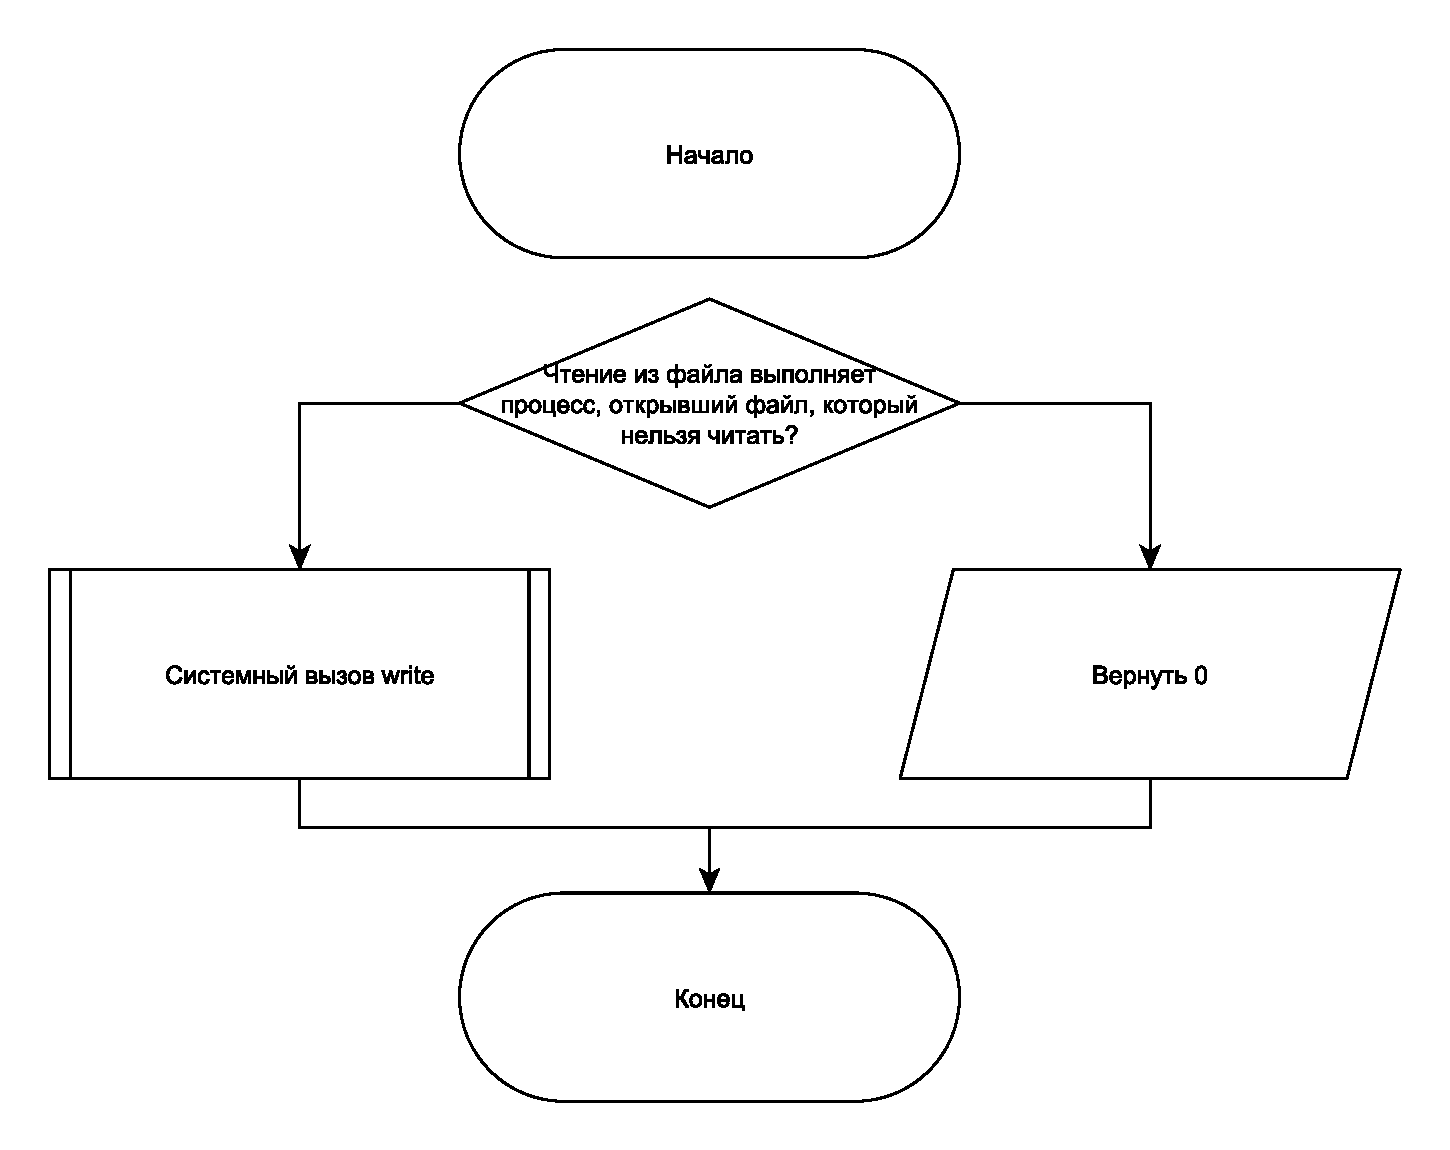
\includegraphics[scale=0.5]{img/third.eps}
	\caption{Алгоритм проверки разрешения на удаление файла}
	\label{fig:3}
\end{figure}

\section{Алгоритм проверки разрешения на чтение из файла}

На рисунке~\ref{fig:4} приведена схема алгоритма проверки разрешения на чтение из файла.

\begin{figure}[H]
	\centering
	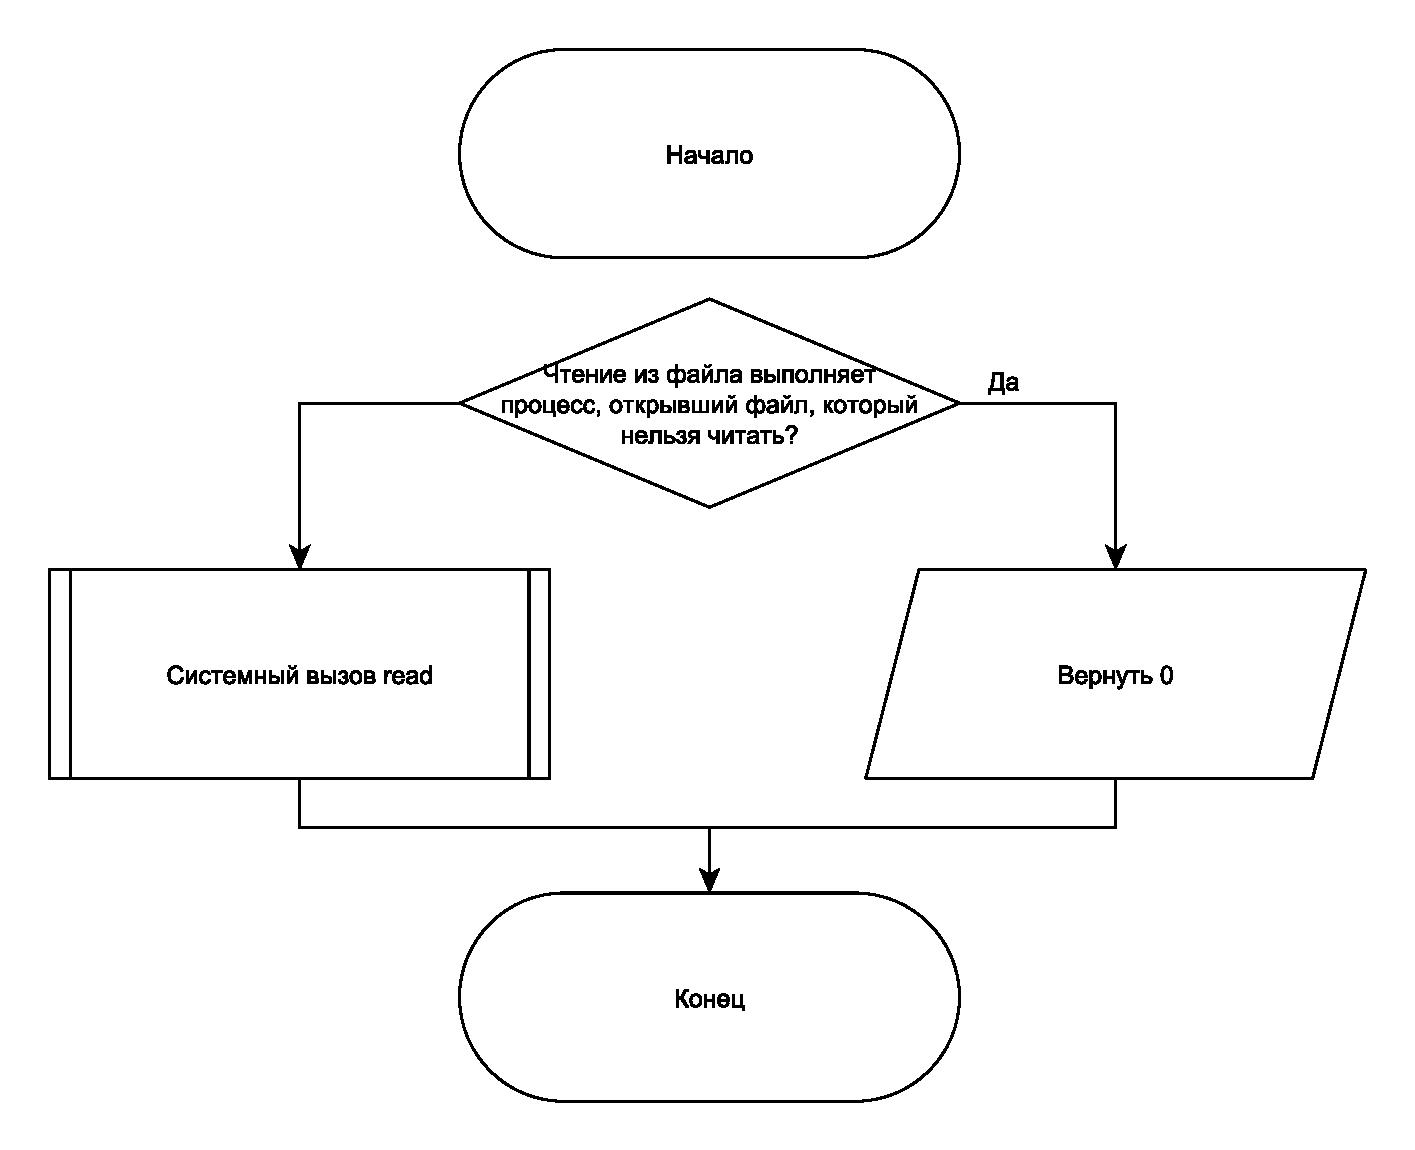
\includegraphics[scale=0.5]{img/fourth.eps}
	\caption{Алгоритм проверки разрешения на удаление файла}
	\label{fig:4}
\end{figure}
